%Typische Problem  Dreiecksmassig

In der GPU-Programmierung kann mann auch viele Probleme treffen.

\subsection{Dreieckförmige Summation}
Ein typisches Problem ist Bloksummation. Aus der Beschreibungen der Operationen Multiplikationen der Matrize mal Vektor und Sparsematrize  mal Vektor beruhen obige Operationen auf Vektormultiplikationen, die schließlich ein Summierungsverfahren in jedem Block enthalten. Blocksummation in einzigen Thread ist nicht effizient. Die einführende Algorithmus: Dreieckförmige Summation lautet wie Fig.\ref{Dreieck} . In erst Schritte werden 2n und 2n+1 Elements des Produktvektors Cs in jeweilig Threads summiert. In zweiter Schritte werden 4n und 4n+2 Elements summiert. Bis BlockSize/2 Schritte erhalt man endlich Ergebnisse. 

\begin{figure}[htbp]
%\centering
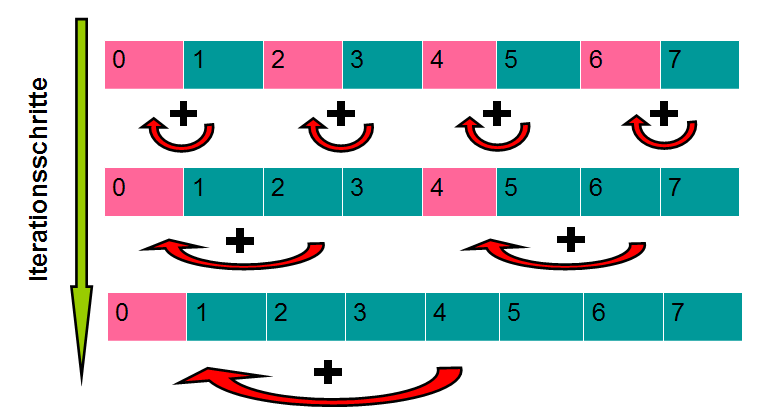
\includegraphics[width=3.5in]{.//pic//dreieck}
\caption{\label{Dreieck}Dreieckförmige Summation. Von Oben nach Unter zeigt}
\end{figure}

Beispiel Code sieht folgende aus,

%Dreieckmassig code zeigen
\begin{verbatim}
#define BLOCK_EXP 9
#define DEF_BLOCKSIZE 1 << BLOCK_EXP
short offset = 1;
for (short i = 1;i < BLOCK_EXP; i++) {
    short old = offset;
    offset <<= 1;
    if (threadIdx.x % offset == 0) {
        Vs[threadIdx.x] += Vs[threadIdx.x
        										+ old];
    }
    __syncthreads();
}
if (threadIdx.x == 0) {
    out[0] = Vs[0] + Vs[offset];
}
\end{verbatim}
